\documentclass[aps,prl,reprint,superscriptaddress,nofootinbib]{revtex4-2}
\usepackage{amsmath,amssymb,graphicx,bm}
\usepackage[colorlinks=true,linkcolor=blue,citecolor=blue,urlcolor=blue]{hyperref}
\newcommand{\D}{\mathcal D}
\newcommand{\E}{\mathbb E}
\newcommand{\ket}[1]{|#1\rangle}
\begin{document}
\title{First-click time scales of a monitored Dicke critical state: a calculation and its prior-art boundary}
\author{Research working note}
\noaffiliation
\hypersetup{pdftitle={First-click time scales of a monitored Dicke critical state: a calculation and its prior-art boundary},pdfauthor={Research working note}}
\date{October 29, 2026}
\begin{abstract}
The time until the first detected photon need not have a single characteristic scale. For a quartic critical soft mode monitored through its position, we derive matched asymptotics for the survival probability and its moments. At large dimensionless monitoring strength $d$, the median is proportional to $d^{-1}$, whereas the mean is proportional to $d^{-3/4}$. A dilute set of records survives until $d^{-1/2}$ and controls moments above order $1/2$. Deterministic propagation checks these predictions, and finite-size Dicke calculations approach the soft-mode distribution. Crucially, the complex-oscillator kernel governing the long records is already contained, including its normalization, in a 2003 atom-optics calculation. Gaussian initial states also have the same exponents. These calculations are therefore retained as a reproducible research note, not presented as a new quantum-critical universality class or a novelty-validated PRL submission.
\end{abstract}
\maketitle

\emph{Question and status.---}A broad first-photon distribution can make a typical observation time differ parametrically from its average. Such behavior is not by itself a new phenomenon: spatially varying loss rates and driven Gaussian cavities already produce algebraic survival intervals followed by exponential decay~\cite{Fedorov,Portugal}. We examine a precise preparation protocol at a finite-size Dicke critical point, derive its moment scaling, and identify its overlap with that earlier work. The distinction between a correct calculation and a new physical mechanism is central to this note.

An initial state is prepared, the Hamiltonian is held fixed, and an ideal detector begins monitoring one loss channel at time zero. We study the first click after this preparation. This is distinct from the interval between successive emissions in a stationary record. In particular, the stationary formula $W(t)=\Pi''(t)/J$ for an interarrival density is not the first-event density $-\Pi'(t)$~\cite{Portugal}. No detector inefficiency or background counts are included.

\emph{Soft-mode calculation.---}Consider
\begin{equation}
 h=\frac{P^2}{2}+\frac{Q^4}{4},\qquad
 \partial_\tau\rho=-i[h,\rho]+d\D[Q]\rho,
 \label{eq:model}
\end{equation}
where $[Q,P]=i$ and $\D[L]\rho=L\rho L^\dagger-\{L^\dagger L,\rho\}/2$.
The initial state $\psi_0$ is the even ground state of $h$. With
\begin{equation}
 h_{\rm eff}=h-\frac{id}{2}Q^2,
 \quad S_d(\tau)=\|e^{-ih_{\rm eff}\tau}\psi_0\|^2,
 \label{eq:survival}
\end{equation}
the first-click density is $-S'_d(\tau)$ and
\begin{equation}
 \E[\tau^r]=r\int_0^\infty \tau^{r-1}S_d(\tau)\,d\tau,
 \qquad r>0.
 \label{eq:moments}
\end{equation}
Let $f(Q)=|\psi_0(Q)|^2$ and $f_0=f(0)>0$. Matched asymptotics at fixed $r$ gives
\begin{equation}
\E[\tau^r]\sim
\begin{cases}
 A_r d^{-r}, & 0<r<\tfrac12,\\
 \dfrac{\sqrt\pi f_0}{4}d^{-1/2}\log d, & r=\tfrac12,\\
 C_r d^{-r/2-1/4}, & r>\tfrac12,
\end{cases}
\label{eq:main}
\end{equation}
where
\begin{align}
 A_r&=\Gamma(1+r)\int_{\mathbb R}f(Q)|Q|^{-2r}\,dQ,\\
 C_r&=rf_0\int_0^\infty u^{r-1}K(u)\,du,\\
 K(u)&=\frac{\sqrt{2\sqrt2\pi}}
 {\sqrt{\sinh(\sqrt2u)+\sin(\sqrt2u)}}.
 \label{eq:kernel}
\end{align}
The median satisfies $\tau_{50}\sim s_{50}/d$. Its coefficient is defined by $F_0(s_{50})=1/2$, with $F_0$ given below. Numerical ground-state quadrature yields
\begin{align}
 f_0&\simeq0.56015,\quad s_{50}\simeq3.05846,\\
 \E[\tau]&\sim3.55394\,d^{-3/4},\qquad
 \E[\tau^2]\sim9.08648\,d^{-5/4}.
 \label{eq:constants}
\end{align}
These are asymptotic coefficients, not fits to a finite-$d$ power law.

\begin{figure*}[t]
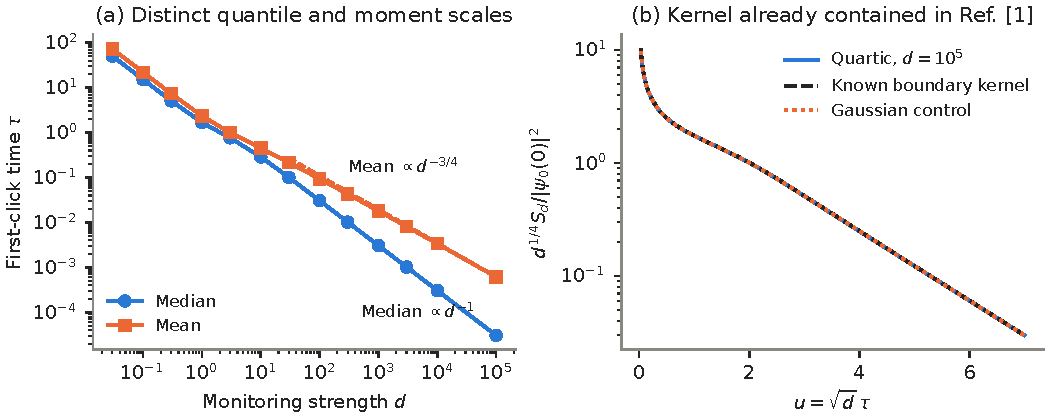
\includegraphics[width=\textwidth]{../figures/first_click.pdf}
\caption{First-click statistics in the effective model. (a) Deterministic propagation from the quartic ground state; dashed lines show the asymptotes in Eq.~\eqref{eq:constants} and $s_{50}/d$. Finite-$d$ corrections to the scaled mean remain visible even at $10^5$. (b) The normalized long-record survival approaches the known kernel~\cite{Fedorov}. An ordinary harmonic-oscillator Gaussian initial state gives the same limit. The quartic data use 9601 grid points at the largest $d$. These results verify the calculation, not its novelty.}
\label{fig:first}
\end{figure*}

\emph{Origin of the two scales.---}At fixed $s=d\tau$ the potential and kinetic evolution are subleading, giving
\begin{equation}
 S_d(s/d)\longrightarrow F_0(s)
 =\int f(Q)e^{-sQ^2}\,dQ.
 \label{eq:frozen}
\end{equation}
For $d^{-1}\ll\tau\ll d^{-1/2}$, only positions near $Q=0$ survive:
\begin{equation}
 S_d(\tau)\sim f_0\sqrt{\frac{\pi}{d\tau}}.
 \label{eq:tail}
\end{equation}
No-click conditioning narrows the wavefunction to width $(d\tau)^{-1/2}$. The kinetic phase becomes order one when $d\tau^2\sim1$. Freezing the coordinate beyond this point incorrectly predicts a divergent mean.

Set $Q=d^{-1/4}y$ and $\tau=d^{-1/2}u$. Then
\begin{equation}
 \frac{h_{\rm eff}}{\sqrt d}
 =\frac{p_y^2-iy^2}{2}+\frac{d^{-3/2}}4y^4.
 \label{eq:boundary}
\end{equation}
The leading local initial amplitude is constant. Writing $\Omega_c=e^{-i\pi/4}$, its evolved value is
\begin{equation}
 \chi(y,u)=\frac{\exp[-i\Omega_c\tan(\Omega_cu)y^2/2]}
 {\sqrt{\cos(\Omega_cu)}}.
 \label{eq:chi}
\end{equation}
Consequently,
\begin{equation}
 S_d(u/\sqrt d)\sim f_0d^{-1/4}\int|\chi(y,u)|^2dy
 =f_0d^{-1/4}K(u).
 \label{eq:match}
\end{equation}
The kernel obeys $K(u)\sim\sqrt{\pi/u}$ at small $u$ and
$K(u)\sim\sqrt{4\sqrt2\pi}\,e^{-u/\sqrt2}$ at large $u$.
Thus records of probability weight $d^{-1/4}$ last until $d^{-1/2}$, although fixed quantiles occur at $d^{-1}$.

For $r<1/2$, integration of Eq.~\eqref{eq:frozen} gives $A_r$. For $r>1/2$, Eq.~\eqref{eq:match} gives $C_r$. At $r=1/2$, the intermediate integral is proportional to
$d^{-1/2}\int_{d^{-1}}^{d^{-1/2}}d\tau/\tau$, giving the logarithm in Eq.~\eqref{eq:main}. This is a matched-asymptotic derivation supported by numerical propagation; a uniform operator bound allowing all microscopic limits and moment integrals to be exchanged has not been established here. The multiplication operator $Q$ has no normalizable zero vector, but that fact alone would not establish such a bound.

\begin{figure*}[t]
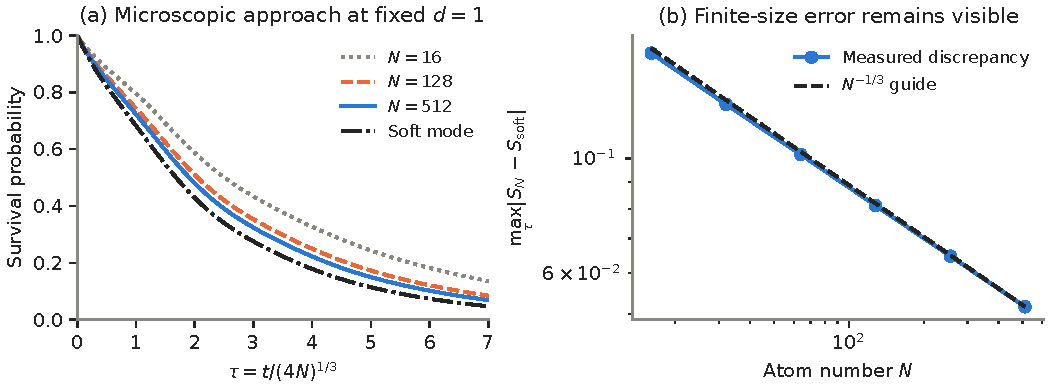
\includegraphics[width=\textwidth]{../figures/microscopic.pdf}
\caption{Microscopic checks at fixed effective strength $d=1$. (a) Direct Dicke no-click propagation approaches the quartic prediction as $N$ increases. (b) The maximum curve discrepancy on $0\leq\tau\leq7$ decreases approximately as the displayed $N^{-1/3}$ guide; this line is not a proof of an error exponent. Numerical cutoff changes are much smaller than these finite-size differences.}
\label{fig:micro}
\end{figure*}

\emph{Dicke realization and finite-size checks.---}In resonant units, take
\begin{equation}
 H_N=a^\dagger a+J_z+\frac{(a+a^\dagger)J_x}{\sqrt N},
 \qquad L=\sqrt{2\kappa}\,a,
 \label{eq:dicke}
\end{equation}
with $J=N/2$. The coupling is the closed-system critical value in this convention. The initial state is the finite-$N$ ground state of $H_N$, and the bare cavity loss is then switched on. Open Dicke noise and finite-size criticality are extensively studied~\cite{DallaTorre,LiWang}; the present protocol concerns this prepared initial state, not the stationary open critical state.

The leading Holstein--Primakoff expansion gives a soft coordinate $q$ with
\begin{equation}
 H_{\rm soft}=\frac{p^2}{2}+\frac{q^4}{16N}+\cdots,
 \qquad a_{\rm soft}=\frac q2+\cdots.
\end{equation}
Define $\ell=(4N)^{1/6}$. The substitutions
\begin{equation}
 q=\ell Q,\quad t=\ell^2\tau,\quad
 d=\frac{\kappa\ell^4}{2}=2^{1/3}\kappa N^{2/3}
 \label{eq:mapping}
\end{equation}
give Eq.~\eqref{eq:model} at fixed $d$ as $N\to\infty$.
The noise scale differs from a damping time inferred solely from $\kappa^{-1}$, because the jump matrix element grows with the critical coordinate. This scaling observation does not make the boundary kernel a specifically critical phenomenon.

Taking the effective large-$d$ limit after the soft-mode limit predicts
\begin{align}
 t_{50}&\sim3.85342\,\kappa^{-1}N^{-1/3},\\
 \E[t]&\sim4.74394\,\kappa^{-3/4}N^{-1/6}.
 \label{eq:physical}
\end{align}
The hierarchy $N^{-2/3}\ll\kappa\ll1$ is suggested by the two scales. Equation~\eqref{eq:physical} is not a claim about arbitrarily strong loss at fixed $N$, nor a proved uniform result for every path through this hierarchy. Hard-mode contributions and the momentum part of $a$ must remain negligible.

We evolve the full no-click state with $H_N-i\kappa a^\dagger a$, in the permutation-symmetric spin sector, for $N=16,32,64,128,256,512$ and $d=0.3,1,3$. At $d=1$, the maximum survival discrepancy from the soft-mode curve decreases from $0.1603$ at $N=16$ to $0.0516$ at $N=512$ (Fig.~\ref{fig:micro}). The scaled gap increases from $0.9627$ to $1.0446$, toward the quartic value $1.0871$. Increasing the cavity cutoff from 48 to 64 at $N=256,512$ changes the computed survival by at most $1.1\times10^{-9}$. This resolves truncation error; it does not remove finite-size error. Microscopic time integrals saved with these runs are truncated and are not used as complete means.



The bare-loss prescription is appropriate to an engineered rotating-frame model. A zero-temperature equilibrium bath coupling to dressed excitations can leave the physical ground state invariant. The present calculation must not be read as ground-state radiation from such an equilibrium bath. Nor does it predict general preparation-ramp statistics or a steady-state interarrival law.

\emph{Controls and prior-art identity.---}The exponents do not require a quartic critical state. For an ordinary harmonic ground state,
$f(Q)=\sqrt{\omega/\pi}\,e^{-\omega Q^2}$, Eq.~\eqref{eq:frozen} becomes
$F_0(s)=\sqrt{\omega/(\omega+s)}$, and $s_{50}=3\omega$. Its large-$d$ boundary dynamics is still Eq.~\eqref{eq:boundary} without the quartic correction, giving the same moment exponents. A smooth odd initial state, with $f(Q)\propto Q^2$ near zero, instead has an intermediate survival proportional to $(d\tau)^{-3/2}$; the leading mean then scales as $d^{-1}$. Stored odd-state propagation is a control for the role of local initial weight, not an additional claim of a new mechanism.

Even the leading boundary dynamics has a classical stochastic representation. The unnormalized Wigner function obeys
\begin{equation}
 \partial_u W=-p\partial_y W+\frac14\partial_p^2W-y^2W.
 \label{eq:wigner}
\end{equation}
This is random acceleration, $dy=p\,du$, $dp=dB_u/\sqrt2$, with killing rate $y^2$. The local constant density matrix corresponds to a flat, nonnormalized position measure times $\delta(p)$; absorption makes its total weight finite for $u>0$. Equation~\eqref{eq:wigner} does not imply that the full quartic finite-$d$ Wigner function is positive. It does show why the leading exponents are not a witness of nonclassicality.

The decisive prior-art comparison is stronger than a shared exponent. Fedorov \emph{et al.}~\cite{Fedorov} retained atomic motion near a standing-wave node. Their Eq.~(69), at resonance, is
\begin{equation}
 H_F=-\omega_r\partial_X^2-
 \frac{i|\Omega|^2}{2\Gamma}X^2.
\end{equation}
With $\theta=2\omega_rt$ and $d=|\Omega|^2/(2\Gamma\omega_r)$, the scaled generator is exactly the quadratic part of Eq.~\eqref{eq:boundary}. Their Eq.~(78) is Eq.~\eqref{eq:chi}; their Eq.~(84) is
\begin{equation}
 W_{\rm tot}^{(m)}=\frac{d^{-1/4}}{\pi}K(\sqrt d\,\theta).
\end{equation}
The factor $1/\pi$ is their local uniform initial density. It takes the place of $f_0$ in Eq.~\eqref{eq:match}. Their Sec.~7.3.2 also discusses the ultimate localized mode and exponential decay. The metastable population becomes the leading no-emission survival after eliminating the excited state; at finite parameters it is not the full two-component norm.

These exact results occur in the extended JETP publication, not all in the shorter earlier preprint~\cite{Efremov}. Checking only the latter would miss the most direct overlap. The fractional-moment formulas above may organize useful consequences of the known kernel, but the kernel, its kinetic origin, and its exponential cutoff cannot be claimed as new. Finite-$d$ quartic curves and the Dicke parameter mapping are distinct calculations; their present interpretation does not establish a PRL-level advance.

\emph{Reproducibility and conclusion.---}The accompanying scripts use finite differences and Crank--Nicolson propagation for the quartic mode, and sparse matrix exponentiation for the microscopic model. The finest even-state runs use 9601 spatial points on $[-9,9]$ and maximum time step $0.002/\max(1,\sqrt d)$. The integrated emission probability differs from unity by less than $8\times10^{-6}$, and independent flux and survival integrals for the mean agree within $2\times10^{-6}$. Space--time refinement and all raw curves are saved. The known-kernel identity is additionally checked numerically using the original paper's parameters.

The calculation explains how rare no-click records control different moments, with a clear mapping to a Dicke preparation protocol. The same calculation also demonstrates why its strongest proposed novelty does not survive direct comparison with prior work. This note preserves the useful derivation and reproducible evidence without relabeling an established mechanism as a new quantum-critical result.

\bibliography{references}
\end{document}
